\chapter{Demo}\label{cap:demo}
Per illustrare il funzionamento dell'algoritmo insieme ai suoi principali passaggi, è stata realizzata una demo utilizzando la libreria Python \texttt{Gradio}, che consente la creazione di applicazioni web semplici ed intuitive per modelli di machine learning e intelligenza artificiale, in poche righe di codice.

L'interfaccia guida l'utente attraverso tre fasi fondamentali: caricamento dell'immagine, pre-processing e riconoscimento (OCR).

Nella prima fase, l’utente può caricare uno screenshot da elaborare, tramite upload oppure incollandolo direttamente dagli appunti.
\begin{figure}[H]
    \centering
    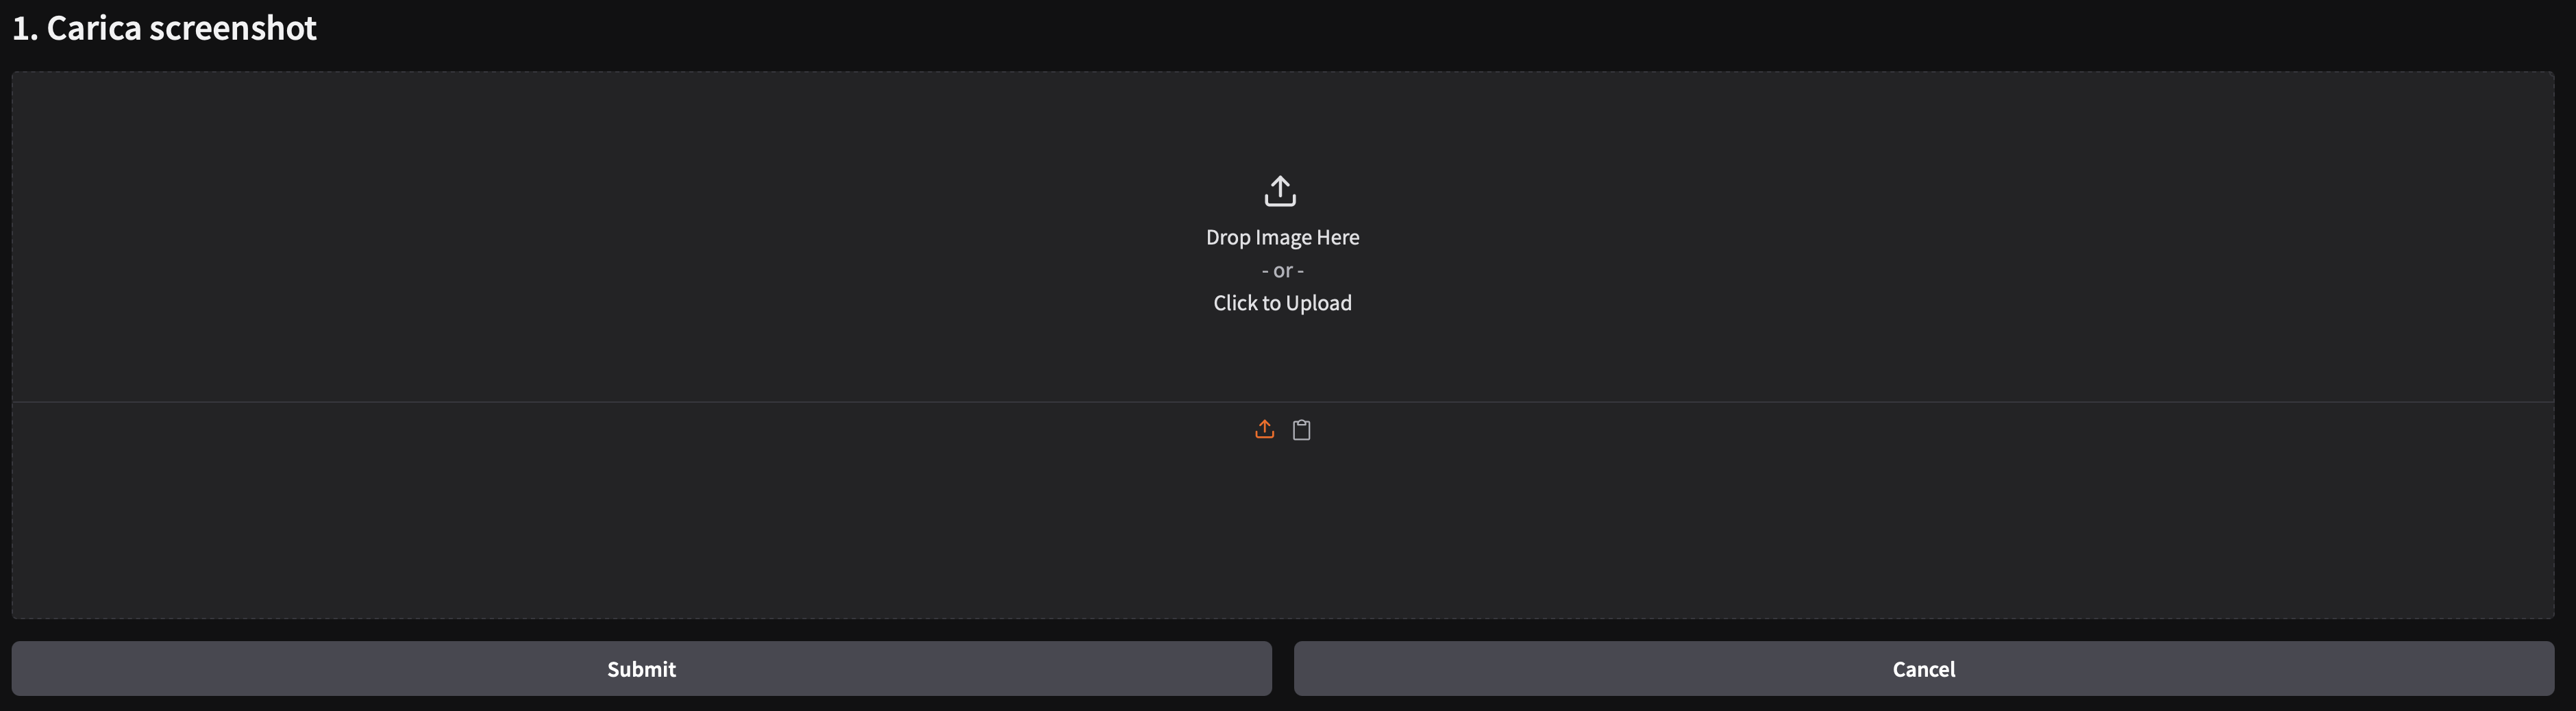
\includegraphics[width=1\textwidth]{images/demo-1fase.png}
    \caption{Interfaccia di caricamento dell'immagine nella demo.}
    \label{fig:demo-1fase}
\end{figure}

Una volta cliccato il pulsante \texttt{Elabora}, avviene l'elaborazione dell'immagine. In output, l'applicazione restituisce due risultati: l'immagine annotata con i bounding box rilevati durante il pre-processing (sovrapposti all'immagine originale) e il testo riconosciuto.

\begin{figure}[H]
    \centering
    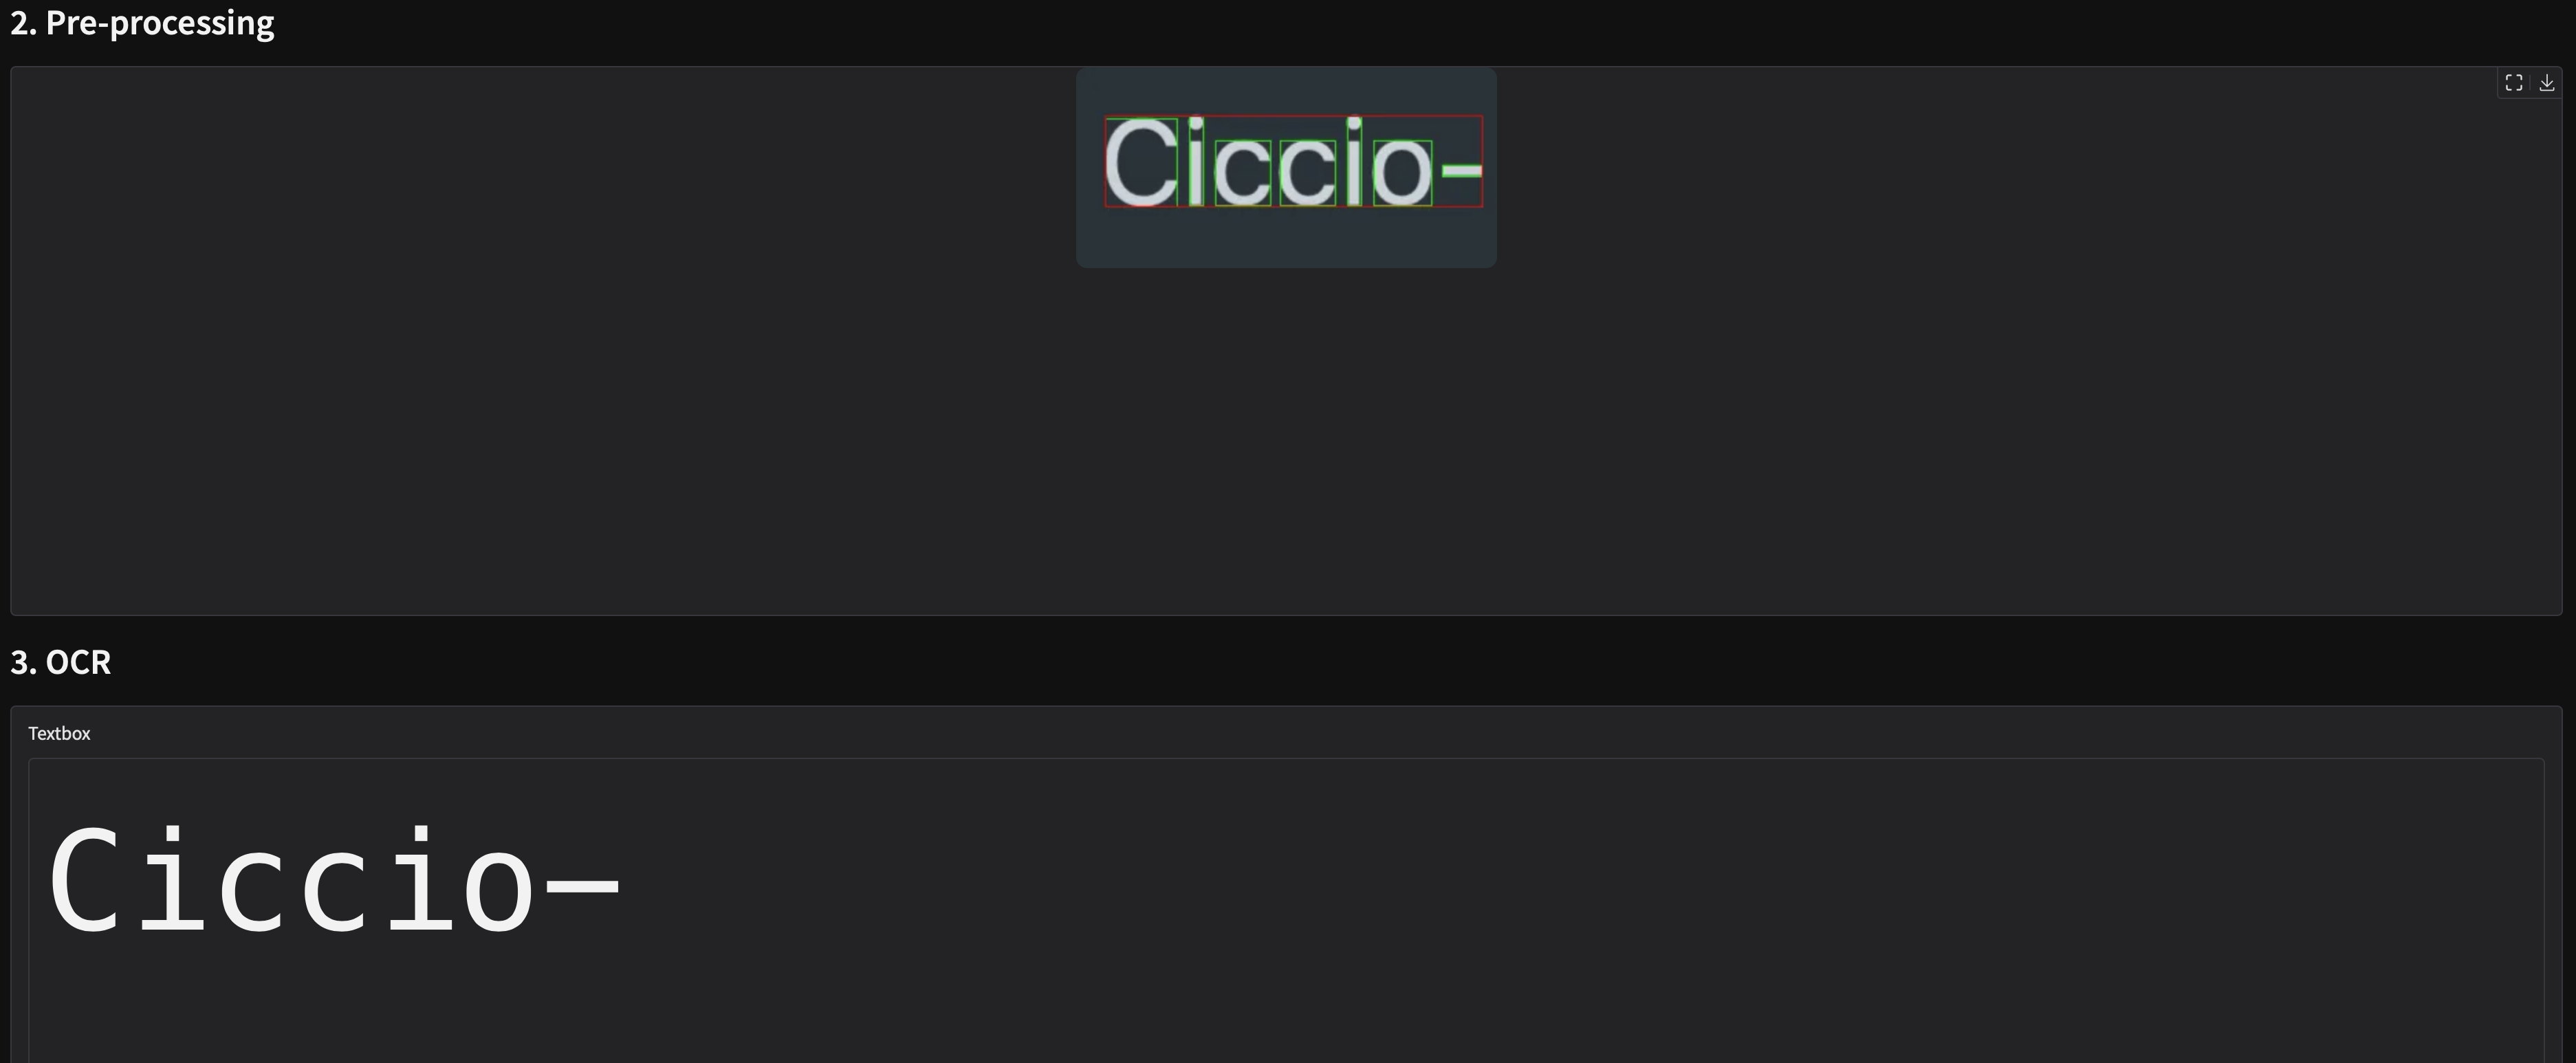
\includegraphics[width=1\textwidth]{images/demo-23fase.png}
    \caption{Output dell'immagine preprocessata e del testo riconosciuto.}
    \label{fig:demo-23fase}
\end{figure}